\documentclass[conference]{IEEEtran}
\IEEEoverridecommandlockouts
% The preceding line is only needed to identify funding in the first footnote.
% If that is unneeded, please comment it out.
\usepackage{cite}
\usepackage{amsmath,amssymb,amsfonts}

%\usepackage{graphicx}
\usepackage{textcomp}
\usepackage{xcolor}
\usepackage{tikz}
\usepackage{pgfplots}
\usepackage{pgfplotstable}
\usepackage{rtsched}
\usepackage{threeparttable}
\usepackage{csvsimple}
\usepackage{booktabs} % For \toprule, \midrule and \bottomrule
\usepackage{siunitx} % Formats the units and values
%\usepackage[hidelinks]{hyperref}
\usetikzlibrary{patterns,calc,arrows}
\usepackage[utf8]{inputenc}
\usepackage[T1]{fontenc}
\usepackage{pgf}
\usepackage{amsmath}
\usepackage{bm}
\usepackage{url}
%\usepackage{algorithm}
%\usepackage{algpseudocode}
\def\UrlBreaks{\do\/\do-}
\usepackage{breakurl}
%\usepackage[breaklinks,hidelinks]{hyperref}

\newcommand{\mytabcolseplarger}{8.5pt}
\newcommand{\mytabcolseplarge}{6pt}
\newcommand{\mytabcolsepsmall}{3pt}


%\setlength{\textfloatsep}{0pt}
\setlength{\abovecaptionskip}{-3pt} 
\setlength{\belowcaptionskip}{-3pt}

\ifCLASSOPTIONcompsoc
    \usepackage[caption=false, font=normalsize, labelfont=sf, textfont=sf]{subfig}
\else
\usepackage[caption=false, font=footnotesize]{subfig}
\fi

\pgfplotsset{compat=1.15}

\def\BibTeX{{\rm B\kern-.05em{\sc i\kern-.025em b}\kern-.08em
    T\kern-.1667em\lower.7ex\hbox{E}\kern-.125emX}}
\title{Intermediate report : Energy aware memory allocation in real-time systems}

\begin{document}
\maketitle


\section{Introduction}
\label{introduction}

The project's goal is to find a new solution for energy aware memory allocation
in real-time systems. We already know that memory allocation using Core Coupled
Memory (CCM) SRAM helps to increase microcontroller performances
\cite{mem_alloc}. We want to know if this kind of allocation can also reduce
energy consumption for the system. 

\section{Operating mode}

\subsection{Materials}
For this project we will use two different microcontrollers based on the Arm
Cortex-M4 32 bit core. We have a STM32F3 Discovery (STM32F3003VC) and a STM32G4
(STM32G431KB). The intensity during computing is measured with a Nucleo-LPM01A.
We will firstly focus on the STM32F3 performances, the STM32G4 has a different
memory architecture and can run code at higher frequency. This microcontroller
will be used later for comparison with STM32F3. 

\subsection{Intensity measurement with Nucleo-LPM01A}
For the STM32F3 we have to remove the jumper JP3 to allow the consumption
measurement of the board. Then we will branch the STM32F3's VDD pin and GND pin
to the LPM01A on the basic connector CN14 at pins 3 and 1. The two boards are
power supplied with USB cables connected to the computer. However the processor
of the STM32F3 is powered by the LPM01A. So when the code is running we can
obtain directly the intensity graph with the STM32 Cube Monitor PWR application.
\cite{low_power} 

For the STM32G4 we remove the jumper JP1 and we measure the current with the
exact same way. 

\subsection{Obtaining results}
All the test are done the same way to always have the same graph pattern. We
compute the code several times with different memory allocation and frequency.
To separate the different executions we put the processor into stop mode (~60
uA). So we can see picks corresponding to each execution. The first pick is due
to the reset button so we remove it during the data management.
\begin{center}

    \begin{figure*}[htb]
        \centering
        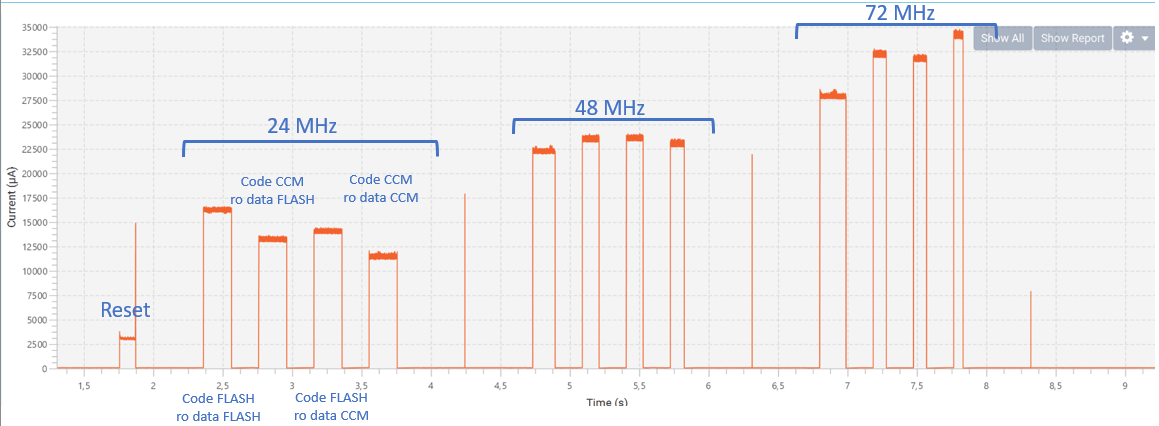
\includegraphics[scale=0.80]{images/pointer_chase_capture_mod.png}
        \caption{Intensity consumption graph for differents pointer chase executions}
        \label{fig:graph_intensity}
    \end{figure*}
\end{center}
Then  The graph can be saved as a .stpm file. This file is an archive containing
one or several .csv files divided into two columns, one with the intensity and
the other with the time. We made a python code to automatically extract the
results from the .stpm file. Our code will browse all the contained .csv files
and will detect all the intensity pics. It will return an excel file where we
can find the average intensity of each pic with their duration. To verify the
execution times we use timers in the STM32F3 code and transmit the execution
time with UART connection. There is a difference of 1 to 2 \% between the time
we mesure on the intensity graph and the duration obtained with timers, however,
the gap between the different measures remains the same with the two procedures.
Moreover, for calculating the energy it is more convenient to measure the
duration when there is a power consumption. 

\subsection{Compilation}
Cube IDE gives a wide range of optimization levels for compilation. We used the
default optimization for release mode. This level of optimization helps to
reduce the space used in memory.

\section{Benchmark}

To verify the microcontroller behavior and have a set of data we used five
benchmarks from "Memory allocation for low-power real-time embedded
microcontroller" \cite{mem_alloc} work and add three from TACle benchmarks
\cite{benchmark}. We specify code inputs and read only data-size. 

\begin{itemize}
    \item Pointer Chase, code: 62B, no inputs, read only : 3.91 KB.
    \item Bubble Sort, code : 1.28 KB, inputs : 3.91 KB, no read only data.
    \item Fast Fourier Transform, code 1 KB, inputs : 4 KB, no read only data.
    \item RSA-Encryption and Decryption, code : 145 and 172 B, inputs : 0.5 KB
    and 4 KB, no read only data.
    \item Kalman Filter, code : 1.62 KB, inputs : 4 KB, no read only data.
    \item Matrix Product, code : 198 B, inputs : 4.68 KB, no read only data.
    \item Sine Lookup Table, code 228 B, inputs : 6.84 KB ,read only : 5.6 KB. 
    \item Dijkstra, code : 532 B, inputs : 6.25 KB, others : 16.26 KB, no read
    only data. 
    \item Fibonacci Recursive : code : 128 B, inputs : 8 B, no read only data. 
    
\end{itemize}

\section{Moving instructions in CCM}
For this part we will analyze the impact of moving instructions in the CCM
instead of Flash memory.

\begin{center}
    \begin{figure*}[htb]
        \centering
        \includegraphics*{plot/code_ccm_energy.pdf}
        \caption[format=hang]{Energy consumption decrease by moving instructions
        from \emph{Flash} to the \emph{CCM-RAM}} \label{fig:code_ccm_energy}
    \end{figure*}
    \begin{figure*}[htb]
        \includegraphics*{plot/code_ccm_intensity.pdf}
        \caption[format=hang]{Average execution intensity decrease over
        frequency by moving instructions from \emph{Flash} to the
        \emph{CCM-RAM}} \label{fig:code_ccm_intensity}
    \end{figure*}
   \begin{figure*}[htb]     
        \includegraphics*{plot/code_ccm_runtime.pdf}
        \caption[format=hang]{Execution time decrease over frequency by moving
        instructions from \emph{Flash} to the \emph{CCM-RAM}}
        \label{fig:code_ccm_intensity}
    \end{figure*}
\end{center}
\clearpage
We measure the energy consumption of a task by integrating the average intensity
during the execution over the execution time. Energy consumption decrease
(\ref{fig:code_ccm_energy}) would be a result of a runtime decrease and an
intensity decrease. In low frequency CCM allows an intensity decrease
(\ref{fig:code_ccm_intensity}) and as no impact on runtime \cite{mem_alloc}.
Then it can explain easily the energy consumption amelioration. However we can
observe that the average intensity increases at high frequencies when moving
code in CCM. In high frequency the FLASH runs more slowly than the processor.
FLASH memory  maximum frequency is 24 MHz on the STM32F3 and the processor can
run at 72MHz. This difference imply some wait states if the cpu ask instruction
when the FLASH is not ready. It explains why runtime is lower in high frequency
(with CCM SRAM there are no wait states). We think that these wait states also
lower the average intensity, because the processor does not consume energy
during these moments. Even if, there is no intensity reduction with CCM in High
frequency (or even an augmentation) the runtime decrease compensate this. Then
we still have an energy consumption decrease by moving code in CCM.

As comparaison we compiled the bubble sort algorithm with another optimization
level. It is the same used in the previous article (\cite{mem_alloc}). It is one
of the lowest level of optimization. It can be used for debugging process.
Optimizing the code have a big impact on our measure. With optimization the
difference between FLASH and CCM is more flagrant. 

\section{Impact on absolute energy}


\begin{table}[h!]
\centering
\begin{tabular}{||c c c c||} 
 \hline
 Algorithm & 24MHz & 48MHz & 72MHz \\ [0.5ex] \hline\hline
 Pointer Chase & 10.826 & 11.852 & 17.320 \\ 
 Bubble Sort & 13.300 & 13.907 & 15.832 \\
 Bubble Sort no opti & 47.238 & 45.317 & 45.361 \\
 RSA decrypt & 5.229 & 5.170 & 5.560 \\
 Kalman & 2.210 & 2.310 & 2.566 \\
 Dijkstra & 42.077 & 42.741 & 44.415 \\[1ex] 
 \hline
\end{tabular}
\caption{Absolute energy (mJ) with instruction in Flash}
\label{energy_tab_code_flash}
\end{table}



\begin{table}[h!]
\centering
\begin{tabular}{||c c c c||} 
 \hline
 Algorithm & 24MHz & 48MHz & 72MHz \\ [0.5ex] \hline\hline
 Pointer Chase & 8.815 & 9.402 & 10.026 \\ 
 Bubble Sort & 11.294 & 10.962 & 10.893 \\
 Bubble Sort no opti & 43.017 & 42.524 & 41.669 \\
 RSA decrypt & 5.239 & 5.166 & 5.469 \\
 Kalman & 2.301 & 2.357 & 2.665 \\
 Dijkstra & 36.318 & 35.189 & 34.828 \\[1ex] 
 \hline
\end{tabular}
\caption{Absolute energy (mJ) with instruction in CCM SRAM}
\label{energy_tab_code_ccm}
\end{table}

When instructions are in the FLASH memory the energy increase with the
frequency. However, when the code is running from CCM SRAM, the energy remain
constant and can even be lowered in high frequency. This observation can be
counter-intuitive, but it is shown that high frequency execution can reduce
energy consumption \cite{pwr_clock}. This is not true in the case of FLASH
execution because the wait states imply an overhead consumption. Because the
energy is the product between intensity, runtime and voltage we can conclude
that, wait states increase execution time more than they reduce the intensity
(voltage remain constant). 

\[\Delta E = \frac{I_1 \frac{n_1}{f_1} - I_2 \frac{n}{f_2}}{I_1 \frac{n_2}{f_1}} \]
In the case of no wait states $n_1 == n_2$
\[\Rightarrow \Delta E = 1 - \frac{f_1}{f_2} \frac{I_2}{I_1}\]
With $n$ the amount of clock cycles to execute the task.

The variation of energy is null if the intensity grows proportionally with the
frequency. In our case the intensity follows: $I(f) = a + b.f^\alpha$ with
$\alpha \in ]0,1[$. When code is running from CCM there is no wait states so n
remains constant over the frequency. Then, the above formula is true. However,
when code runs from FLASH :

\[\Delta E = 1 - \frac{I_2}{I_1} \frac{n_2}{n_1} \frac{f_1}{f_2}\]
\[n_2 = n_1 + n_1.w = n_1(1+w) \] 
\begin{center}
    with $w$ the wait state ratio $w >= 0$   
\end{center}
\[\Delta E = 1 - (1+w)\frac{I_2}{I_1} \frac{f_1}{f_2}\]

With the $(1+w)$ factor the intensity growth has to be even more small between
frequencies. With $f_2 = 72 MHz, f_1 = 24 MHz$ and $w = 0.4$ the intensity ratio
has to be inferior to 2.14 to do not have energy increase. With no wait states it would be 3.


\bibliographystyle{unsrt}
\bibliography{bibliography}

\end{document}

\endinput
%%
%% End of file `elsarticle-template-harv.tex'.
